.% -*- mode: latex; mode: linkd; mode: auto-fill; mode: flyspell;-*-
% Index
% (@> "Introduction")
% (@> "Collaboration")
%   (@> "Advantages of collaboration")
%    (@> "Knowledge sharing")
%    (@> "Richer forms of communication")
%    (@> "Share Resources")
%   (@> "Classification of CSCW Systems")

\chapter{Collaborative modelling}
\label{chap-four}

% (@file :file-name "thesis.tex")

% (@* "Introduction")
The objective of Coglaborate is to provide a collaborative modeling
environment for the cognitive science community. It does so by
mounting ACT-R on the Biobike infrastructure. The system currently
supports collaboration asynchronously. This means that a certain
researcher can develop a model and share it with his colleague, who
can work on that model separately and share it with other individuals.

% This chapter discusses the advantages provided by a shared environment
% such as Coglaborate. It also tries to provide a framework for the future
% development of Coglaborate, by providing the means that we used to come
% up with the requirements for this system.

This chapter starts off with a discussion about collaborative
systems. Which is then followed by a discussion about biobike, its
objectives and which part of the spectrum of the collaborative systems
it fits into. 

\section{Collaboration}
% (@* "Collaboration")
%explain why is collaboration required. 
Collaboration is the key to building large structures in almost all
human endeavors be it in the fields of either the arts or
sciences. Collaboration permits breaking down large unwieldy tasks
into more manageable chunks of work. It permits sharing of knowledge
and resources. Computer networks have provided us with a means of
communication between users of computers. This as a result has led to
an area of research that studies how computers can help users
communicate their ideas through computers and therefore use computers
as a means of collaboration, this field is commonly known as Computer
Supported Collaborative Work (CSCW).

\subsection{Advantages of collaboration using computers}
% (@* "Advantages of collaboration")
% Advantages of using computers in collaboration: Describe why you
% need this
We have three outcomes as a result of using computers to support
collaboration. They assist is sharing knowledge, for example consider
a Wiki. No other means that we currently know of would enable us to
share knowledge as freely and easily. They enhance communication
by allowing us to share richer content like video with each
other. Finally they allow us to share resources such as processing
power and storage capacity. Each of these outcomes have their
advantages that are discussed in detail below.

% (@* "Knowledge sharing")
The ability to share knowledge through computers helps us save
time. For example if a researcher develops a model of a certain
phenomenon on a computer and shares it with the community. Some other
person working on an extension of the project would save the time
taken to build this part of the model in the first place. And since we
are sharing knowledge, collaboration through computers lends it self
easily to be used as a pedagogical tool. For instance consider an
author of a textbook. He can easily create content, such as
presentations or write programs to demonstrate concepts, and can share
it off his website. This information can later be used by other
student and teachers to either learn more effectively and to improve
the way they teach respectively. Sharing knowledge also implies
sharing data. Running certain experiments can be time consuming and/or
costly. For example consider weather simulations a researcher in one
lab could simulate a scenario and make the data for the same available
for others doing so would help others working the area save time and
cost by not having to run that experiment again.

% (@* "Richer forms of communication")
Collaboration through means of computer provides us with richer forms
of communication that has not been available to us before. Apart from
allowing audio based communication, it provides us with means for
video based communication. As a result we can communicate with each
other more comprehensibly and that in turn avoids transfer of
ambiguous information. For example we have systems currently that help
us share screens, such systems could be used, for instance, by a
customer to clearly communicate his requirements to a vendor, who may
be in a different geographical area unambiguously. 

% (@* "Share Resources")
The ability to tie up computers together allows us to share
resources. This could either be in the form of hardware, where a power
server or servers are shared by many people or in the form of human
resources where people from different geographical locations can
collaborate effectively.

% 1) Easier to share knowledge:
%    a) Talk about sharing data,
%    b) code,
%    c) reuse of knowledge
% 2) Communication
%    a) Provides communication: wiki, 
% 3) Repository of knowledge
%    a) Store old knowledge
% 4) Hardware sharing
%    a) More powerful hardware at a common place
%    b) Cost change

\section{Classification of CSCW systems}
% (@* "Classification of CSCW Systems")

According to \cite{journals/iwc/Rodden91} there are two
characteristics of all CSCW systems namely, the form of interaction
and the geographical nature of the users. 

The form of interaction can be described as the method by which users
of a groups working together interact. This could either be
synchronously where every member of a group contributes in real time
an example of such a situation is brain storming. Another form of
interaction is asynchronous interaction. In such a form of interaction
the members of the group with one another with out the presence of
other members of the group. An example of this can be a group of
students collaborating with each other on a homework problem via a
message board.

The geographical nature of the users describes if the users interact
with each other remotely for example consider the case of developing
the linux kernel, developers and testers working on the kernel worked
with each other from geographically disparate locations. It could
also describe if the users are co-located, an example of this could be
users using a meeting room system like Colab\cite{Stefik:1987:BCU}. 

\begin{figure}[htp]
  \caption{Classification of CSCW systems\cite{journals/iwc/Rodden91}}
  \centering
  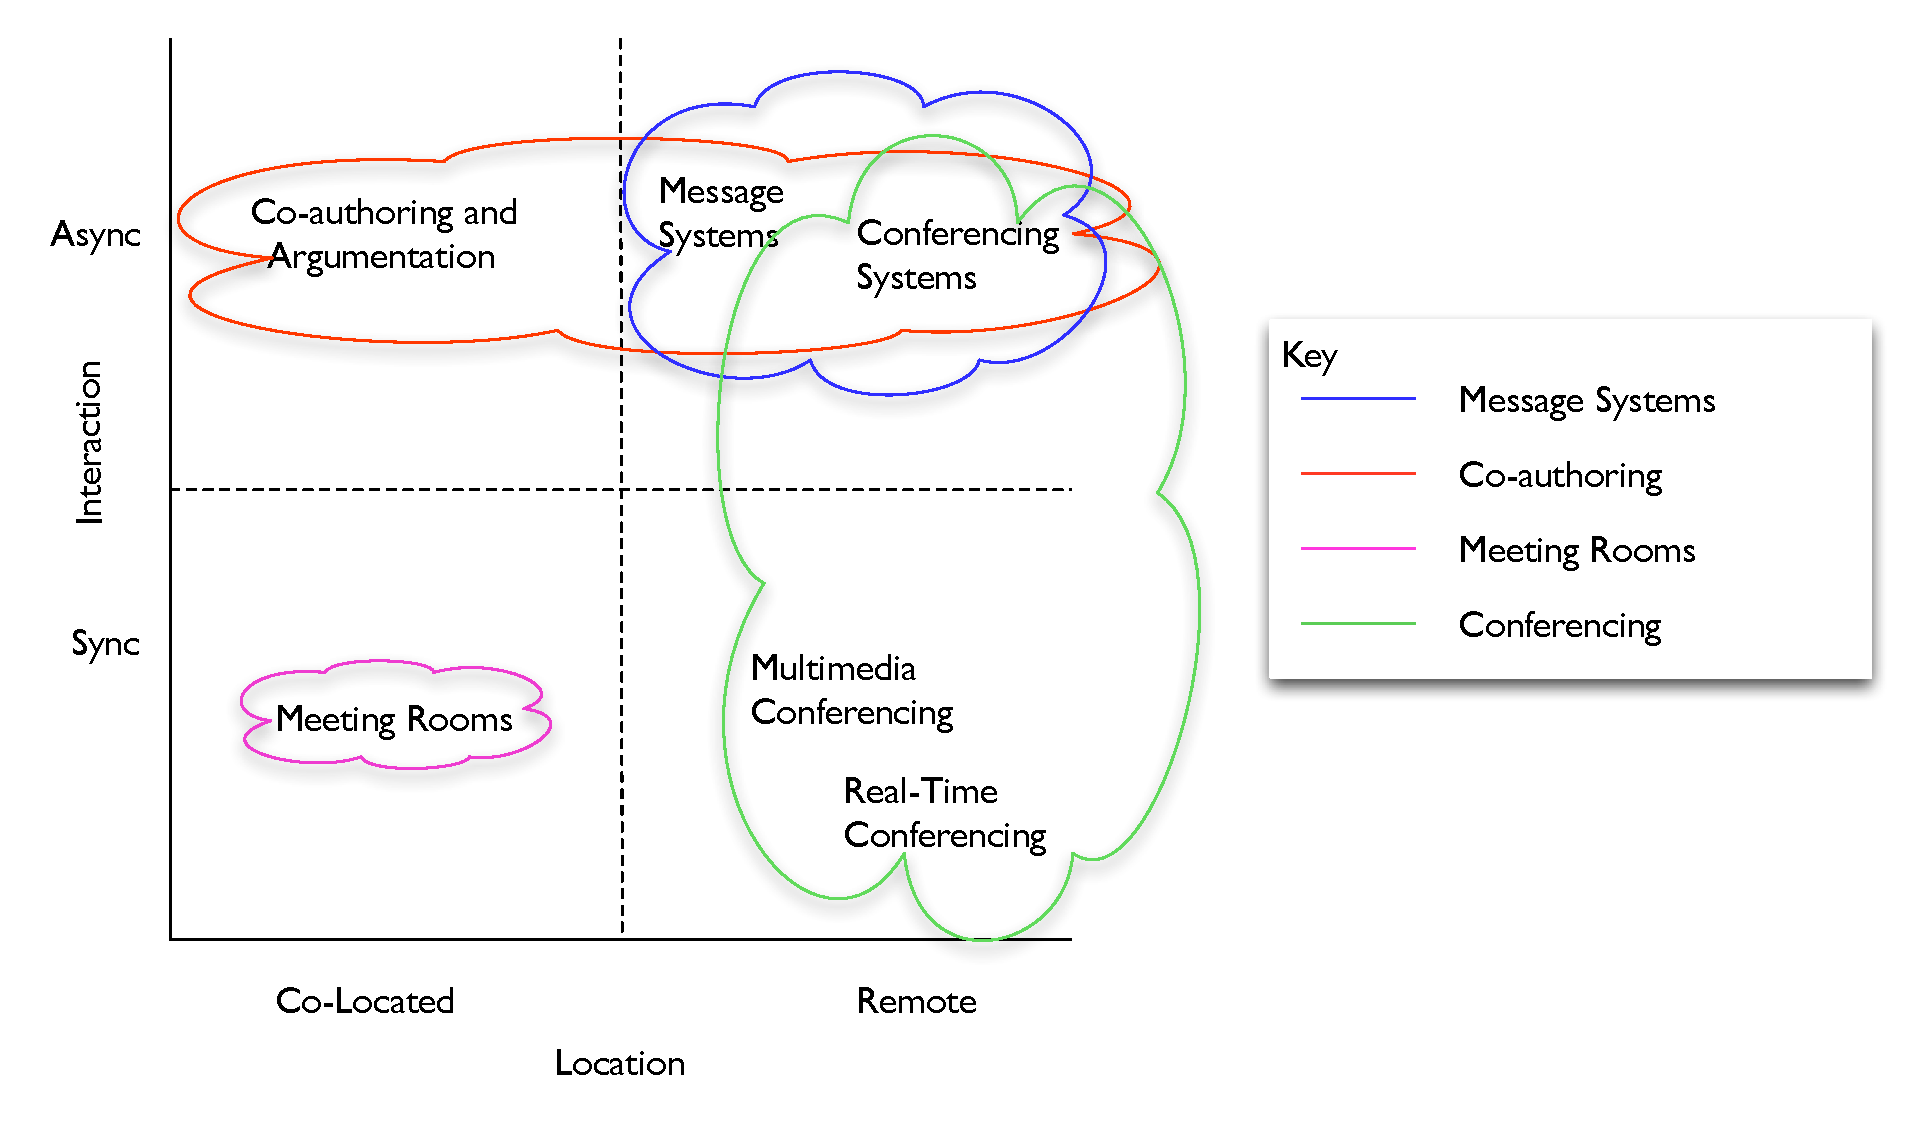
\includegraphics[width=140mm]{CSCWClass.eps}
  \label{CLASS_CSCW}
\end{figure}

\subsection{Message Systems}

Message systems derive their origins from e-mail based systems. The
factor that differentiates message systems from email based systems is
that message systems try to attach more semantic data to the messages
they process. Most of these systems use the object model to represent
messages. To instantiate messages the user fills in data context
specific data into slots, this data is used by the system to carry out
further processing by the system. Example of message systems include
COSMOS\cite{conf/cscw/BowersC88} and Information Lens\cite{Malo87a}. 

COSMOS represented research being carried out in the European CSCW
community. COSMOS was a project in the UK to design and develop a
configurable message system that supported structured group work. The
system was developed with a focus on specifying the users
communicative work in the form of participants actions. Group activity
tasks were represented in the system using the concept of
\emph{communication
  structures}(CS)\cite{conf/cscw/BowersC88}. Communication structures
were further described using a structure definition language(SDL). The
tasks that a COSMOS system was capable of carrying out was defined by
the communication structures defined in the system. The COSMOS system
also defines roles for users or agents, message objects, actions,
rules and actions in context of the work being carried out. Any
communication activity by the user is instantiated when the user
creates an instance of a communication structure. The user does this
by filling in the data required by the communication
structure. Further communication occurs by an exchange of messages
between users who compose a specific role mentioned in the
communication structure.

The Information lens on the other hand take a less formal
approach\cite{journals/iwc/Rodden91}. The aim of the author to develop
information systems that minimized information overload on the users
of the system that was caused by the amount of messages that were sent
to a user. The key ideas that defined Information lens were


\begin{itemize} 
  \item \emph{ Use of semi-structured messages to represent data:} The messages were represented as a set of semi-structured data
  called frames. A frame was a template that included information for
  date, time, place, organizer and any other unstructured data. This
  idea played an important role because; semi-structured messages make
  it easier for the computer to parse messages, according to informal
  studies conducted by the author of the paper\cite{Malo87a} people do
  most of their processing on a set of unstructured information and
  finally providing semi-structured fields enables authors to put in
  more context related information.

\item \emph{The use of production rules:} The system used sets of
  production rules each of which might contain multiple levels of
  reasoning that specify the reasoning of messages.

\item \emph{Use of specialized editors for creating and editing
    message templates and productions: } The authors of the system
  attempted to make the system more user friendly by providing
  multiple editors to create and edit message templates and
  productions.
\item \emph{Use of frame inheritance:} Using frame inheritance in
  messages allows messages to be specialized very easily
\item \emph{Introducing the system slowly to the users:} The authors
  believed that the introduction and evolution of a group work system
  can be useful if it is introduced slowly to users and encouraging
  users to switch to the system by rewarding users who switch to the
  system by providing additional benefits.
\end{itemize}

The message templates consisted of forms having fields where
information could be filled. The messages were edited using a display
oriented editor. The users constructed the IF part by specifying the
conditions that were required by a rule to satisfy condition by
combining specific conditions using logical operators like and, or and
not. The users used message handling primitives like move, delete,
save, etc. to specify the action to be taken on that message.

\subsection{Conferencing systems}
Conferencing systems found their advent in the 1970s when the US
government was looking for a way to deal with emergencies. EMISARI\cite{Hilt78a}

(Emergency Management Information System and Reference Index) was
the result of this effort. It consisted of two main ideas that even
today form the back bone of current conferencing systems. This model
of communication allowed users to interact through a shared
information space, but at the same time it allowed user to interact
individually with one another. 
\subsection{Meeting Rooms Systems}

\subsection{Co-authoring and Argumentation Systems}

\section{Biobike}

% This section can contain the introduction and objectives of biobike
% and where biobike fits in with the rest of the collaborative systems.












